\documentclass{beamer}
\mode<presentation>{
\usetheme{Madrid}
%\setbeamertemplate{caption}[numbered]
%\setbeamertemplate{footline} % To remove the footer line in all slides uncomment this line
\setbeamertemplate{footline}[page number] % To replace the footer line in all slides with a simple slide count uncomment this line
\setbeamertemplate{navigation symbols}{}
}

\usepackage{amsmath}
\usepackage{graphicx}
\usepackage{mathtools}
\usepackage[font={scriptsize}]{caption}
\graphicspath{{img/}}

\title[Estocasticidad en circuitos gen\'eticos]{Modelos estoc\'asticos de circuitos gen\'eticos}
\author{Luis Alberto Guti\'errez L\'opez}
\institute[Uniandes]{Universidad de los Andes\\
Departamento de F\'isica\\
\medskip
}
\date{Marzo 9 de 2016}

\begin{document}

\begin{frame}
\titlepage
\end{frame}

\begin{frame}
\frametitle{Expresi\'on gen\'etica}

\begin{columns}[c]
\column{.7\textwidth}

\begin{figure}[p]
    \centering
    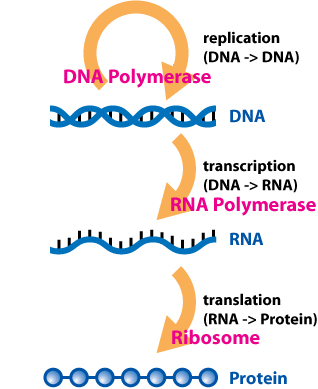
\includegraphics[width=0.5\textwidth]{dogma.jpg}\\
    \tiny Tomado de: \url{https://en.wikipedia.org/wiki/Central_dogma_of_molecular_biology}.
\end{figure}

\column{.3\textwidth}

\begin{figure}[p]
    \centering
    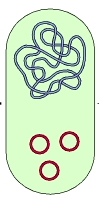
\includegraphics[width=0.3\textwidth]{plasmid.png}\\
    \tiny \cite{cooper00}.
\end{figure}

\end{columns}

\begin{figure}[p]
    \centering
    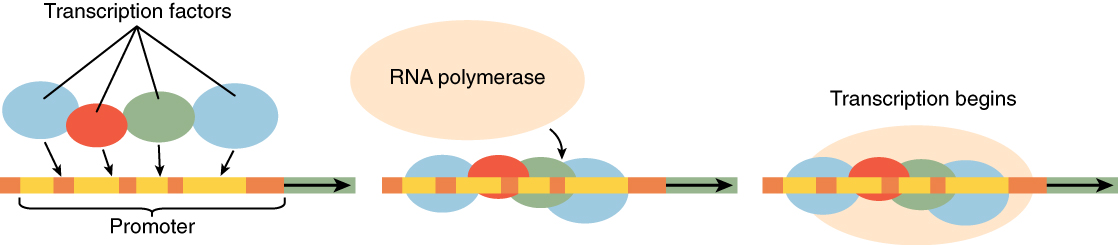
\includegraphics[width=0.8\textwidth]{tf1.jpg}\\
    \tiny Tomado de \url{http://oerpub.github.io/epubjs-demo-book/content/m46036.xhtml}.
\end{figure}
\end{frame}

\begin{frame}
\frametitle{Circuitos gen\'eticos}

\begin{figure}[p]
    \centering
    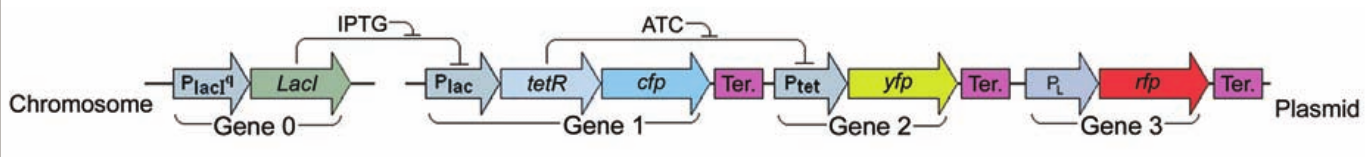
\includegraphics[width=0.9\textwidth]{circuitex.png}\\
    \tiny \cite{pedraza05}.
\end{figure}

\begin{figure}[p]
    \centering
    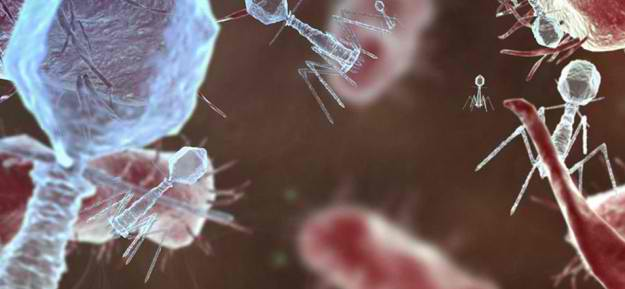
\includegraphics[width=0.2\textwidth]{phageim.jpg}\\
    \tiny Tomado de: \url{phages.org}.
\end{figure}

\begin{figure}[p]
    \centering
    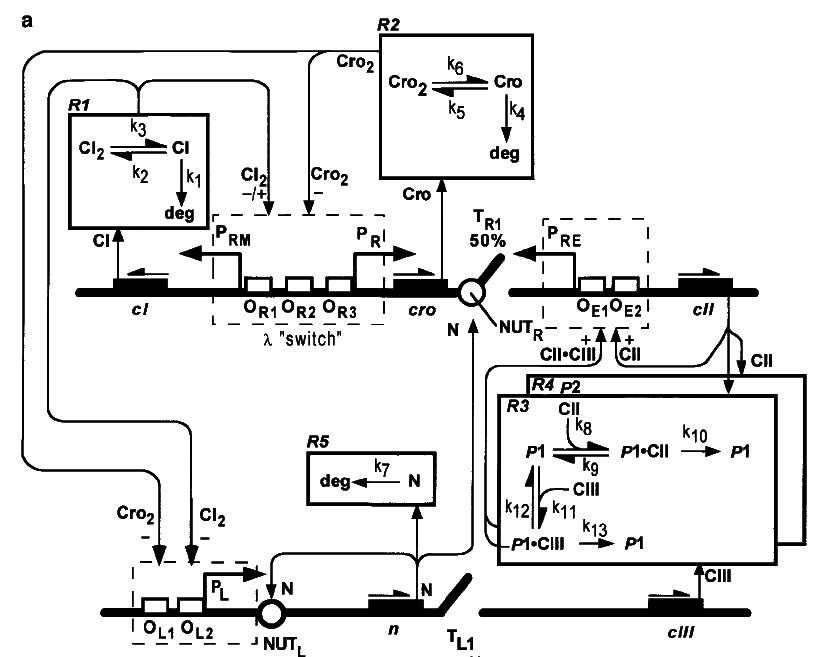
\includegraphics[width=0.35\textwidth]{lambdacirc.png}\\
    \tiny \cite{arkin98}.
\end{figure}

\end{frame}

\begin{frame}
\frametitle{Ruido en circuitos gen\'eticos}
\begin{itemize}
\item Fluctuaciones aleatorias en expresi\'on gen\'etica.
\item En transcripci\'on y traducci\'on: Colisiones aleatorias entre mol\'eculas que se encuentran en bajo n\'umero (Intr\'inseco).

Para \textit{E. coli} en promedio

$$\langle r\rangle_s \approx 5 \text{ ARNs}$$
$$\langle p\rangle_s \approx 3000 \text{ prote\'inas}$$

\item Otros factores como la divisi\'on celular y la variablidad del ambiente (Extr\'inseco).
\begin{align*}
\eta_X &= \frac{\sigma_X}{\langle X \rangle}.\\[1.5ex]
\nu_X &= \frac{\sigma^2_X}{\langle X \rangle}.
\end{align*}
\end{itemize}
\end{frame}

\begin{frame}
\frametitle{Manifestaciones del ruido}
\begin{figure}[p]
    \centering
    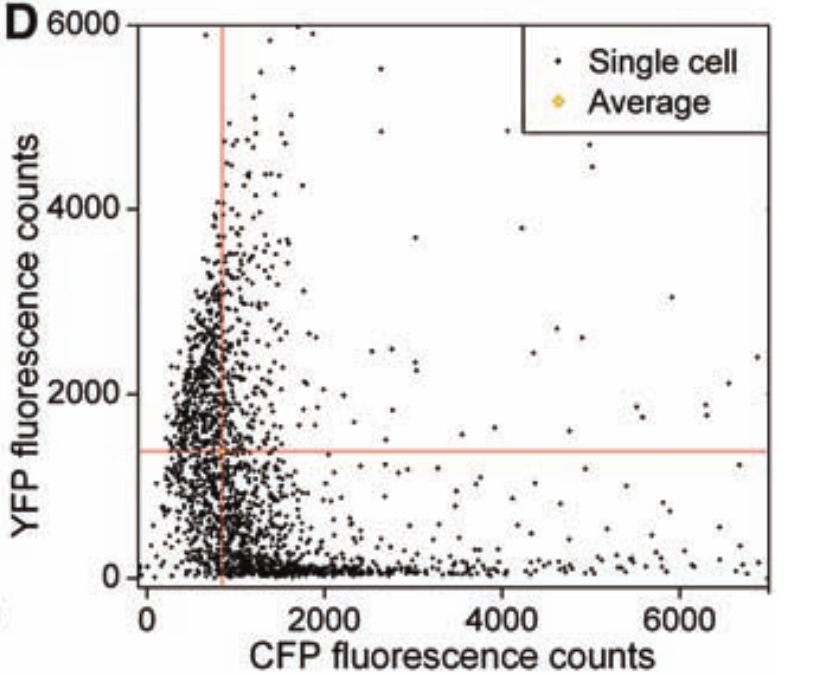
\includegraphics[width=0.5\textwidth]{noiseGFP.png}\\
    \tiny \cite{pedraza05}.
\end{figure}
\end{frame}


\begin{frame}
\frametitle{Estrategias ante el ruido}
\hspace{20 mm} \textbf{Robustez} \hspace{40 mm} \textbf{Variabilidad}
\begin{columns}[c]
\column{.5\textwidth}
\begin{figure}[p]
    \centering
    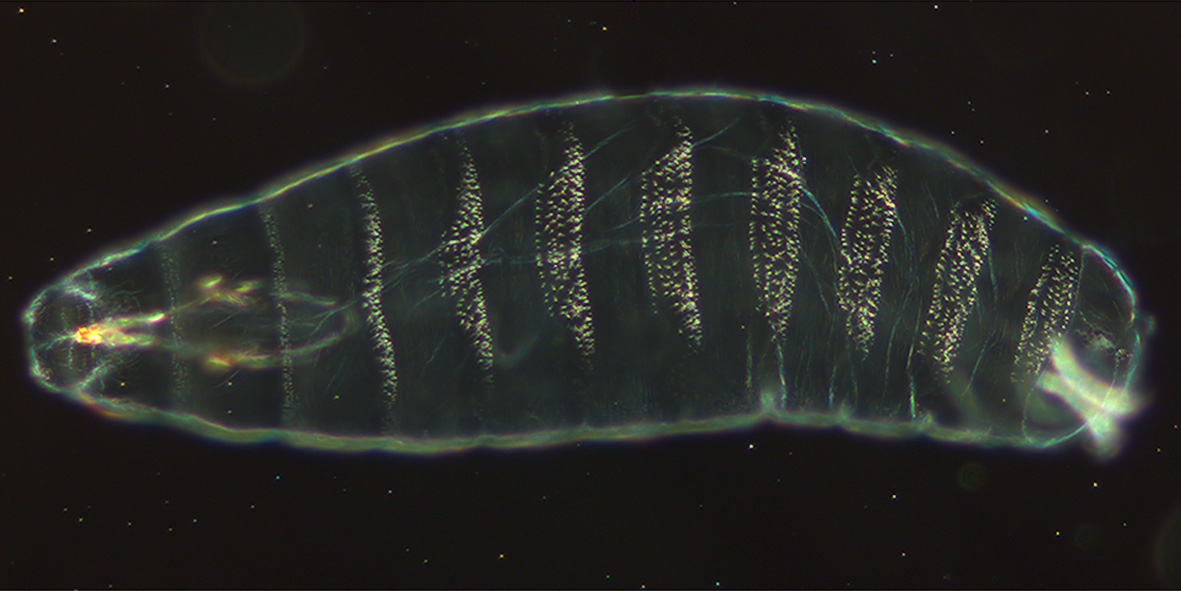
\includegraphics[width=0.9\textwidth]{drosophila.jpg}\\
    \tiny Tomado de: \url{https://en.wikipedia.org/wiki/Drosophila_embryogenesis}.
\end{figure}

\column{.5\textwidth}
\begin{figure}[p]
    \centering
    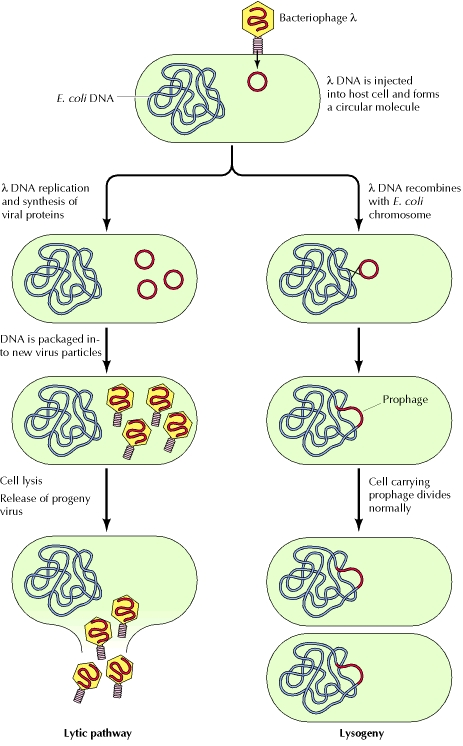
\includegraphics[width=0.7\textwidth]{lambda.jpg}\\
    \tiny \cite{cooper00}.
\end{figure}
\end{columns}
\end{frame}

\begin{frame}
\begin{figure}[p]
    \centering
    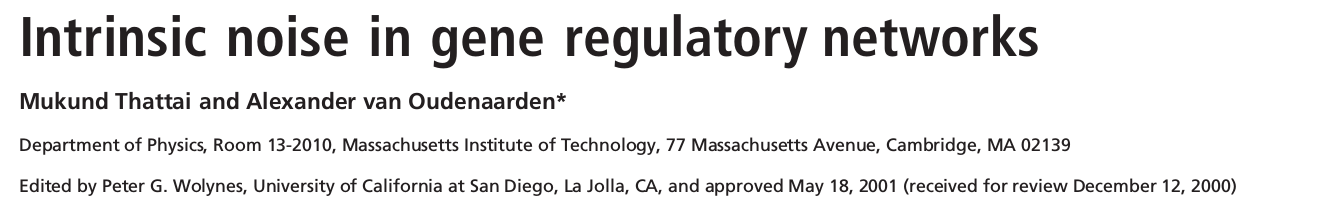
\includegraphics[width=1\textwidth]{title.png}\\
    \tiny \cite{thattai01}.
\end{figure}
\begin{columns}[c]

\column{.5\textwidth}
\begin{figure}[p]
    \centering
    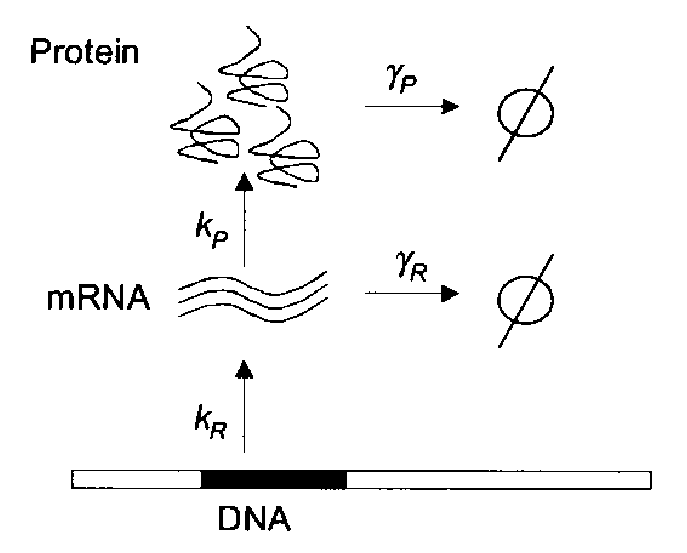
\includegraphics[width=0.5\textwidth]{expressionsimple.png}\\
    \tiny \cite{thattai01}.
\end{figure}
\begin{align*}
\dot{r}(t) &= k_R - \gamma_Rr(t).\\
\dot{p}(t) &= k_Pr(t) - \gamma_Pp(t).
\end{align*}
\column{0.55\textwidth}
\begin{figure}[p]
  \centering
    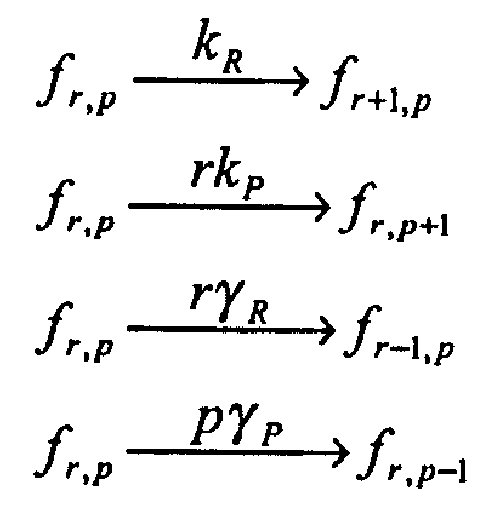
\includegraphics[width=0.4\textwidth]{scheme1.png}\\
    \tiny \cite{thattai01}.
\end{figure}
\begin{align*}
&\frac{d{f}_{r,p}}{dt} = k_Rf_{r-1,p} - k_Rf_{r,p}\\
&+ k_Prf_{r,p-1} - k_Prf_{r,p} + \gamma_R(r+1)f_{r+1,p}\\
&- \gamma_Rrf_{r,p} + \gamma_P(p+1)f_{r,p+1} - \gamma_Ppf_{r,p}.
\end{align*}
\end{columns}
\end{frame}

\begin{frame}
\frametitle{Un s\'olo gen - Resultados}

\begin{columns}[c]
\column{.45\textwidth}
\centering \textbf{Promedio}
\begin{align*}
\langle r \rangle &= \frac{k_R}{\gamma_R}.\\[1.5ex]
\langle p \rangle &= \frac{k_Rb}{\gamma_P}.
\end{align*}
\column{.5\textwidth}
\centering \textbf{Ruido}
\begin{align*}
\nu_r &= \frac{\sigma_r^2}{\langle r \rangle} = 1.\\[1.5ex]
\nu_p &= \frac{\sigma_p^2}{\langle p \rangle} = \frac{b}{1+\eta} + 1 \approx b + 1.
\end{align*}
\end{columns}

\vspace{3 mm}

\begin{equation*}
b \coloneqq \frac{k_P}{\gamma_R}, \quad \eta \coloneqq \frac{\gamma_P}{\gamma_R}.
\end{equation*}

\end{frame}


\begin{frame}
\frametitle{Generalizaci\'on - Ecs. deterministas}

Las ecuaciones

\begin{align*}
\dot{r}(t) &= k_r - \gamma_rr(t),\\
\dot{p}(t) &= k_pr(t) - \gamma_pp(t),
\end{align*}

pueden ser escritas como

\begin{equation*}
\mathbf{\dot{q}} = (A - \Gamma)\mathbf{q}.
\end{equation*}

Donde $\mathbf{q}^T \coloneqq (d, r, p)$ y

\begin{align*}
A \coloneqq \bordermatrix{
  ~ & (d) & (r) & (p) \cr
  (d) & 0 & 0 & 0 \cr
  (r) & k_R & 0 & 0 \cr
  (p) & 0 & k_P & 0 \cr}, \quad \quad
\Gamma \coloneqq \bordermatrix{
  ~ & (d) & (r) & (p) \cr
  (d) & 0 & 0 & 0 \cr
  (r) & 0 & \gamma_R & 0 \cr
  (p) & 0 & 0 & \gamma_P \cr}.\\
\end{align*}
\end{frame}

\begin{frame}
\frametitle{Generalizaci\'on - Ec. maestra}
Se puede realizar en general. Si $\mathbf{q}^T \coloneqq (q_1,q_2,\dots,q_n)$, 
\begin{figure}[p]
    \centering
    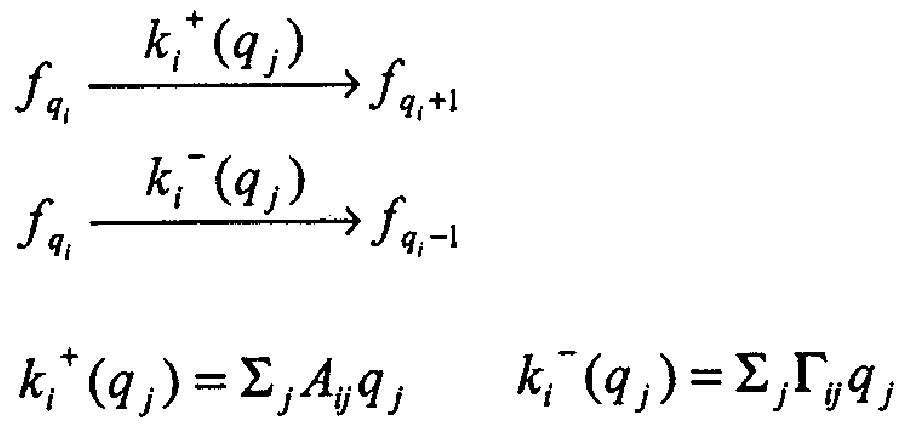
\includegraphics[width=0.6\textwidth]{scheme2.png}\\
    \tiny \cite{thattai01}.
\end{figure}
la ecuaci\'on maestra queda
\begin{equation*}
\dot{f}_{q_i} = \sum_j \left[\left(A_{ij}q_j\right) \left(f_{q_{i-1}} - f_{q_i}\right)\right] + \Gamma_{ii}(q_i+1)f_{q_{i+1}} -\Gamma_{ii}q_if_{q_i}.
\end{equation*}
\end{frame}

\begin{frame}

Al realizar todo el procedimiento obtenemos

$$\left(\mathbf{A} - \mathbf{\Gamma}\right)\langle \mathbf{q} \rangle = 0.$$

$$0 = \left( \left( \mathbf{\Gamma} - \mathbf{A}\right) \nabla\nabla^TF|_1 - A\Theta F|_1 \right) +  \left( \left( \mathbf{\Gamma} - \mathbf{A}\right) \nabla\nabla^TF|_1 - A\Theta F|_1\right)^T,$$ 
$$\Theta_{ij} \coloneqq \delta_{ij}\frac{\partial}{\partial z_i}.$$


\end{frame}

\begin{frame}
\frametitle{Autorregulaci\'on - Modelo}
\begin{figure}[p]
    \centering
    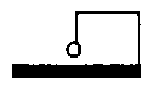
\includegraphics[width=0.2\textwidth]{autorreg.png}\\
    \tiny \cite{thattai01}.
\end{figure}
\begin{columns}[c]

\column{.5\textwidth}
\begin{figure}[p]
    \centering
    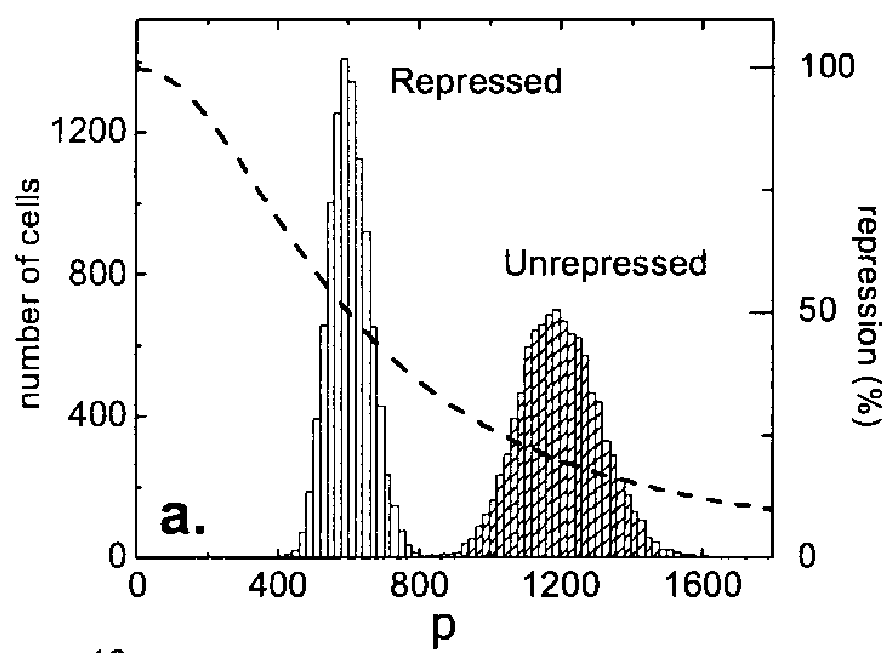
\includegraphics[width=1\textwidth]{graph3.png}\\
    \tiny \cite{thattai01}.
\end{figure}

\column{.5\textwidth}
\begin{itemize}
\item Ecuaci\'on de Hill.
\begin{equation*}
k_R = \frac{k_R^{\text{max}}}{1+(p/K_d)^n}.
\end{equation*}
\item Linearizar alrededor del promedio en estado estacionario.
\begin{equation*}
k_R \approx k_0-k_1p.
\end{equation*}
\begin{equation*}
A = 
\begin{pmatrix}
0 & 0 & 0 \\
k_0 & 0 & -k_1 \\
0 & k_P & 0
\end{pmatrix}.
\end{equation*}
\end{itemize}
\end{columns}
\end{frame}

\begin{frame}
\frametitle{Autorregulaci\'on - Resultados}
\begin{columns}[c]

\column{.45\textwidth}
\centering \textbf{Promedio}
\begin{align*}
%\langle r \rangle &= .\\[1.5ex]
\langle p \rangle &= \frac{1}{1+b\phi} \cdot \frac{k_0b}{\gamma_p}.
\end{align*}

\column{.5\textwidth}
\centering \textbf{Ruido}
\begin{align*}
%\nu_r &= .\\[1.5ex]
\nu_p &= \frac{1-\phi}{1+b\phi} \cdot \frac{b}{1+\eta}+1.
\end{align*}
\end{columns}

\vspace{3 mm}

\begin{equation*}
  b \coloneqq \frac{k_P}{\gamma_R}, \quad \eta \coloneqq \frac{\gamma_P}{\gamma_R}, \quad \phi \coloneqq \frac{k_1}{\gamma_P}.
\end{equation*}

\begin{figure}[p]
    \centering
    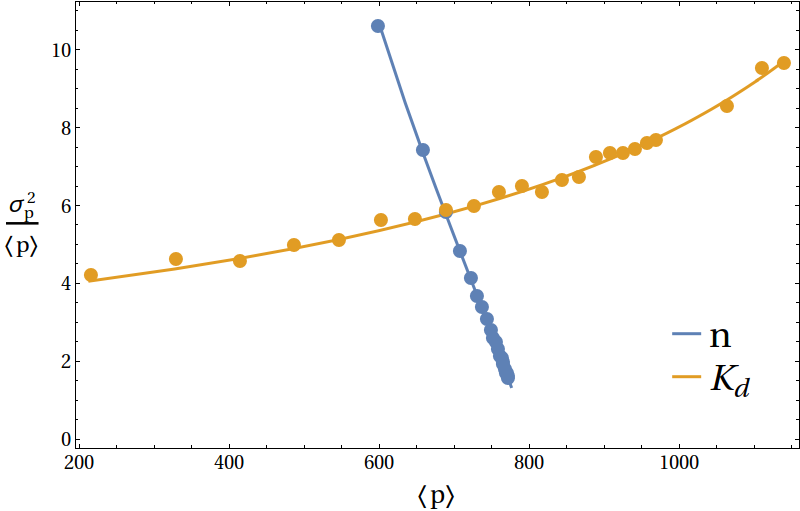
\includegraphics[width=0.5\textwidth]{mas-sim_autorreg.png}\\
\end{figure}

%Problemas
%Hay muchas otras fuentes de ruido que no se consideran.
%Modelo linearizado.
%No sirve para explicar el comportamiento lejos de los puntos fijos si el sistema es no lineal.

\end{frame}

%%%%%%%%%%%%%%%%%%%%%%%%%%%%%%%%%%%%%%%%%%%%%%%%%%%
%TEOREMA DE FLUCTUACION-DISIPACION
%%%%%%%%%%%%%%%%%%%%%%%%%%%%%%%%%%%%%%%%%%%%%%%%%%%
\iffalse
\begin{frame}
\frametitle{Promedio temporal - Teorema de fluctuaci\'on-disipaci\'on}
\begin{figure}[p]
    \centering
    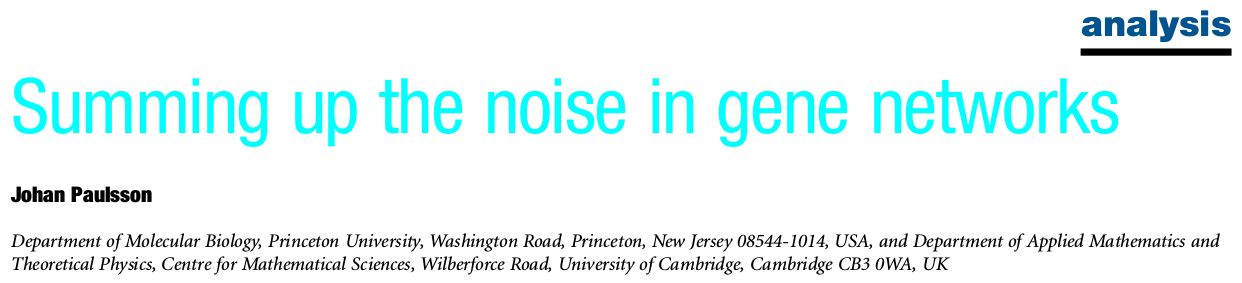
\includegraphics[width=0.75\textwidth]{paulsson04.png}\\
    \tiny \cite{paulsson04}.
\end{figure}

\begin{figure}[p]
    \centering
    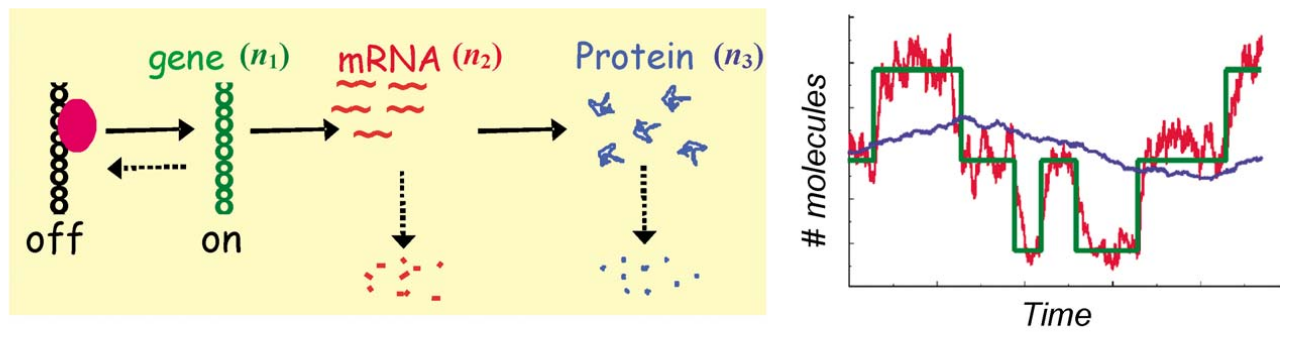
\includegraphics[width=0.75\textwidth]{timeave.png}\\
    \tiny \cite{paulsson05}.
\end{figure}

$$\frac{d\pmb{\sigma}}{dt} = \pmb{A\sigma} + \pmb{\sigma A^T} + \pmb{B}$$

Donde $\pmb{\sigma}$ es la matriz de covarianzas. $\pmb{A}$ y $\pmb{B}$ dependen de las tasas.

\end{frame}

\begin{frame}
\frametitle{Promedio temporal en el ruido}

\begin{figure}[p]
    \centering
    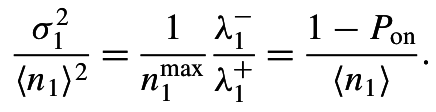
\includegraphics[width=0.4\textwidth]{5d.png}\\
    \tiny \cite{paulsson05}.
\end{figure}

\begin{figure}[p]
    \centering
    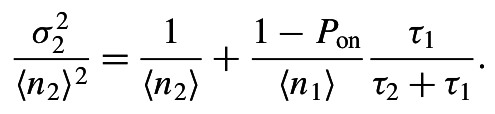
\includegraphics[width=0.4\textwidth]{5r.png}\\
    \tiny \cite{paulsson05}.
\end{figure}

\begin{figure}[p]
    \centering
    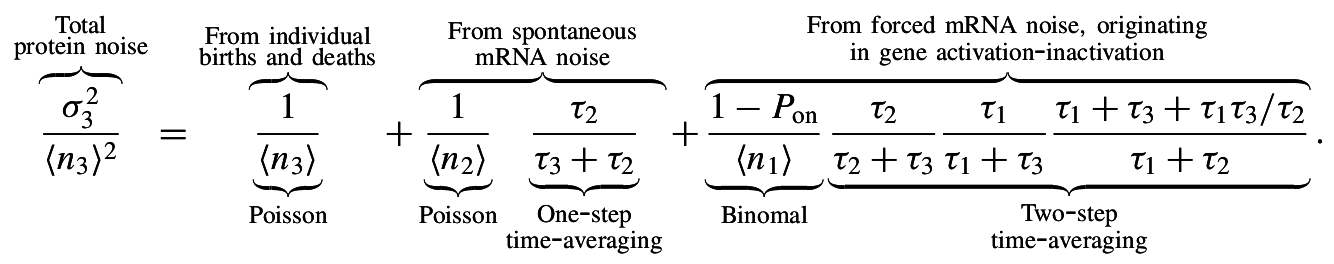
\includegraphics[width=0.75\textwidth]{eqtave.png}\\
    \tiny \cite{paulsson05}.
\end{figure}
\end{frame}
\fi
%%%%%%%%%%%%%%%%%%%%%%%%%%%%%%%%%%%%%%%%%%%%%%%%%%%
%RUIDO GLOBAL Y PROPAGACION DEL RUIDO
%%%%%%%%%%%%%%%%%%%%%%%%%%%%%%%%%%%%%%%%%%%%%%%%%%%

\begin{frame}
  \frametitle{Ruido global y propagaci\'on del ruido}
\begin{figure}[p]
    \centering
    
\includegraphics[width=0.75\textwidth]{pedraza05.png}\\
    \tiny \cite{pedraza05}.
\end{figure}
\begin{figure}[p]
    \centering
    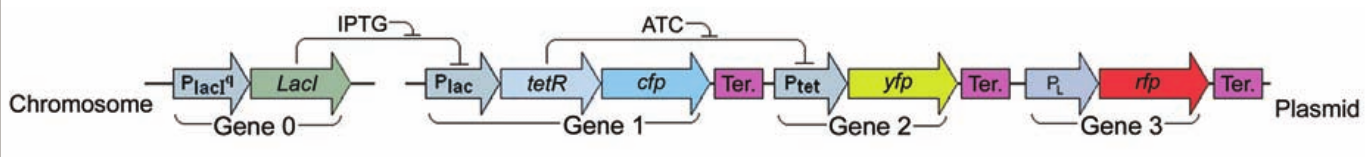
\includegraphics[width=0.75\textwidth]{circuitex.png}\\
    \tiny \cite{pedraza05}.
\end{figure}
\end{frame}

\begin{frame}
  \frametitle{Ecuaci\'on de Langevin - Gen 0}
Ecuaci\'on determinista con t\'erminos de ruido. Para el gen 0
$$\dot{p_0} = k - \gamma p_0 + \mu_0 + \xi_{0}.$$
Los t\'erminos de ruido cumplen:
$$\langle \mu_0 \rangle = \langle \xi_0 \rangle = 0,$$
$$\langle \mu_0(t)\mu_0(t+\tau) \rangle  = 2\gamma (b_0+1) \bar{p_0} \delta(\tau),$$
$$\langle \xi_0(t)\xi_0(t+\tau) \rangle = 2 \gamma \eta_{_G}^2\bar{p_0}^2 \delta(\tau),$$
$$\langle \mu_0(t)\xi_0(t+\tau) \rangle = 0.$$
Luego de hacer el proceso:
$$\eta_0^2=\frac{b_0+1}{\bar{p_0}} + \eta_{0G}^2\coloneqq\eta_{0\,\text{int}}^2+\eta_{0G}^2$$
\end{frame}

\begin{frame}
\frametitle{Ec. de Langevin - Gen 1}
Ahora para el gen 1
$$\dot{p_1} = Nf_1(p_{0}) - \gamma p_1 + \mu_1 + \xi_1$$
Adem\'as de las anteriores autocorrelaciones, hay que incluir:
$$\langle \xi_0(t)\xi_1(t+\tau) \rangle = 2 \gamma \eta_{_G}^2\bar{p_0}\bar{p_1}\delta(\tau),$$
$$\langle \mu_0(t)\mu_1(t+\tau) \rangle =0.$$
Se obtiene al final
$$\eta_1^2 = \eta_{1\,\text{int}}^2 + \frac{1}{2} H_{10}^2 \eta_{0\,\text{int}}^2 + \eta_G^2\left( 1 + \frac{1}{2} H_{10}^2 - H_{10} \right) + \frac{1}{2} \eta_N^2 $$
\end{frame}

\begin{frame}
\frametitle{Distintas fuentes de ruido y su propagaci\'on}
\begin{figure}[p]
    \centering
    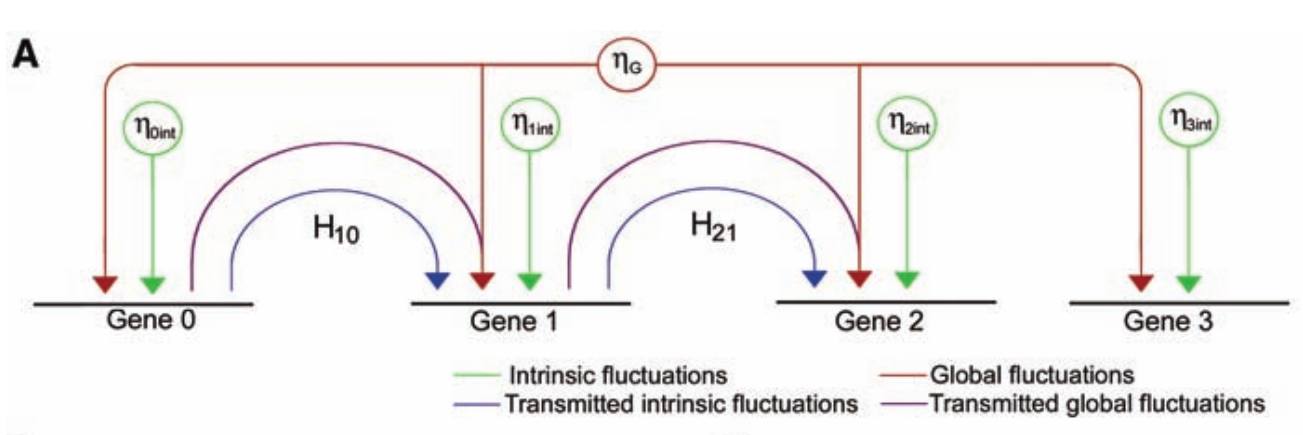
\includegraphics[width=0.75\textwidth]{globalint.png}\\
    \tiny \cite{pedraza05}.
\end{figure}
\end{frame}

\begin{frame}
\frametitle{Ec. de Langevin - Gen 2}
Y similarmente para el gen 2
\begin{align*}
\eta_2^2 &= \eta_{2\,\text{int}}^2 + \frac{1}{2} H_{21}^2 \eta_{1\,\text{int}}^2 + \frac{3}{8}H_{21}^2H_{10}^2\eta_{0\,\text{int}}^2 + \eta_G^2 \left(1 + \frac{1}{2} H_{21}^2\right.\\
&\left.+ \frac{3}{8} H_{21}^2H_{10}^2 - H_{21} - \frac{3}{4}H_{21}^2H_{10} + \frac{1}{2} H_{21}H_{10} \right) + \eta_N^2 \left( \frac{1}{2} + \frac{3}{8}H_{21}^2-\frac{3}{4}H_{21}\right).
\end{align*}
\end{frame}

%Muy chevere porque no se saben con precision las fuentes del ruido global pero a partir de sus estadisticas se puede hallar el ruido

%%%%%%%%%%%%%%%%%%%%%%%%%%%%%%%%%%%%%%%%%%%%%%%%%%%
%MEMORIA Y BURSTING
%%%%%%%%%%%%%%%%%%%%%%%%%%%%%%%%%%%%%%%%%%%%%%%%%%%

%\begin{frame}
%\frametitle{Senescencia}
%\begin{figure}[p]
%    \centering
%    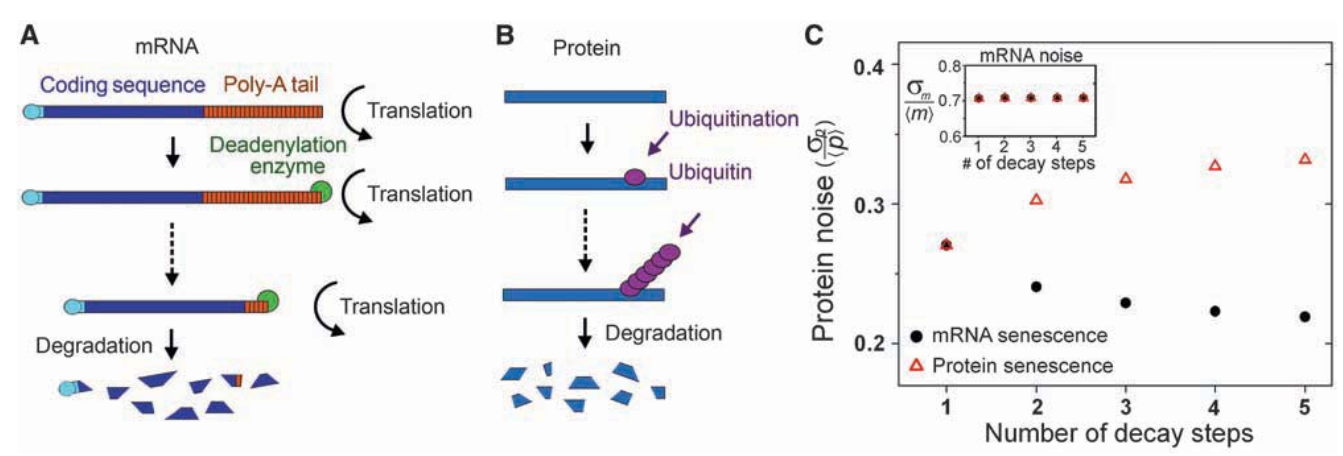
\includegraphics[width=0.9\textwidth]{senes.png}\\
%    \tiny \cite{pedraza08}.
%\end{figure}
%\end{frame}

%\begin{frame}
%\frametitle{Problemas con los ajustes}
%Al considerar distintos factores los ajustes son iguales.

%\begin{figure}[p]
%    \centering
%    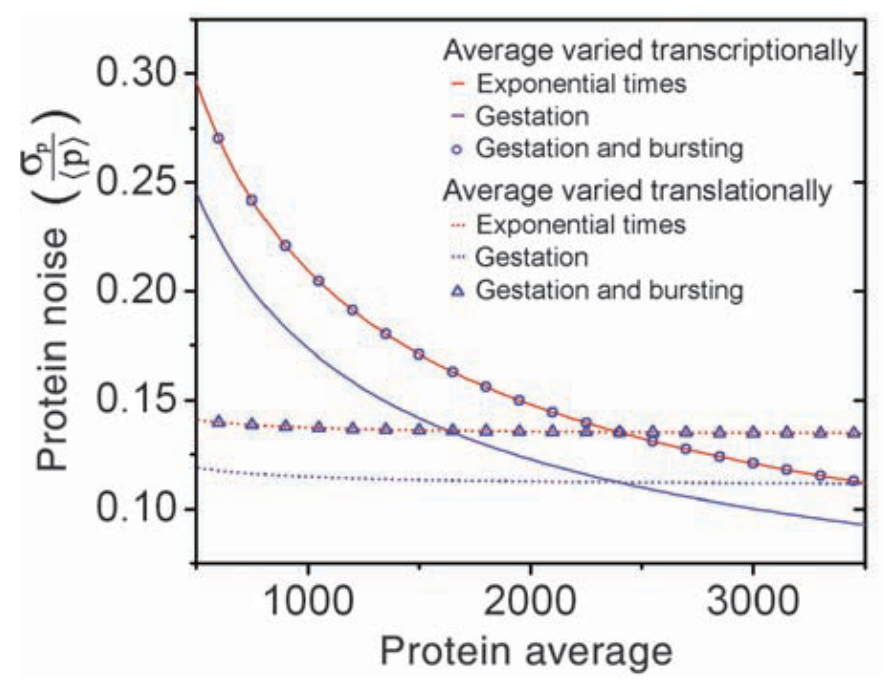
\includegraphics[width=0.5\textwidth]{scaling.png}\\
%    \tiny \cite{pedraza08}.
%\end{figure}
%\end{frame}

%No solo mediante feedback se puede controlar el ruido

\begin{frame}
\frametitle{Ruido por partici\'on}
\begin{figure}[p]
    \centering
    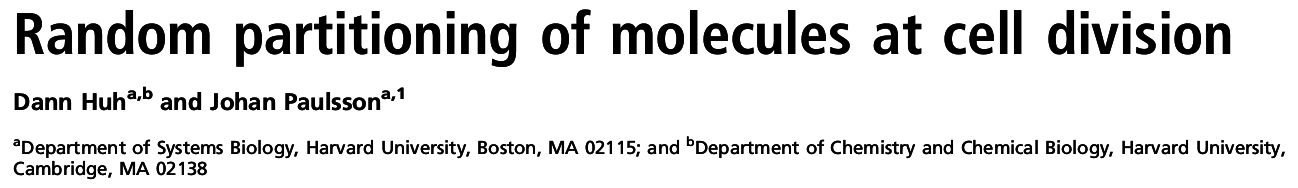
\includegraphics[width=0.75\textwidth]{huh11.png}\\
    \tiny \cite{huh11b}.
\end{figure}

\begin{figure}[p]
    \centering
    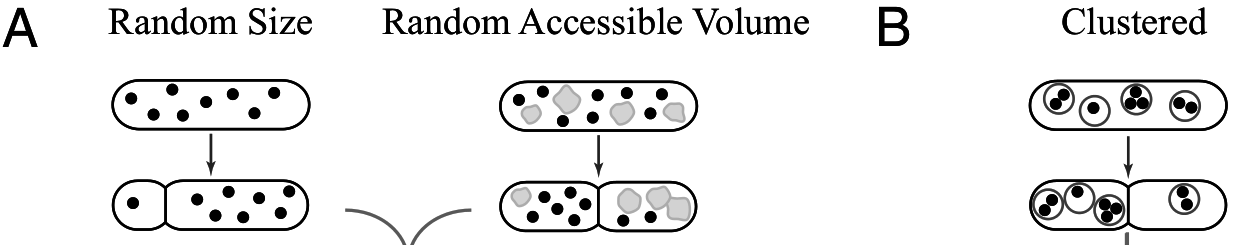
\includegraphics[width=0.8\textwidth]{order.png}\\
    \tiny \cite{huh11b}.
\end{figure}

\begin{figure}[p]
    \centering
    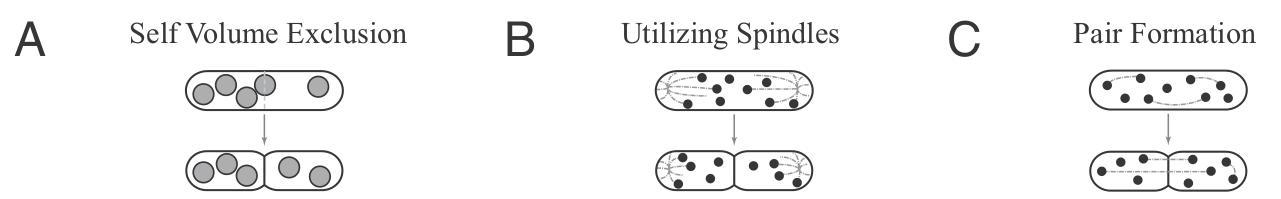
\includegraphics[width=0.85\textwidth]{disorder.png}\\
    \tiny \cite{huh11b}.
\end{figure}

\end{frame}

\iffalse
\begin{frame}
\frametitle{Segregaci\'on ordenada y desordenada}

Para un componente $X$, donde $L$ y $R$ copias se segregan a cada hija:

$$Q_X^2 = \frac{\langle (L-R)^2 \rangle}{\langle X \rangle^2} $$

Para segregaci\'on independiente:

$$Q_X = \frac{1}{\sqrt{X}} $$

Para los mecanismos considerados

$$ Q_X^2 = \frac{A}{X}, \quad \text{donde} \quad 
\begin{cases}
A = 1 \quad \text{para segregaci\'on independiente,}\\
A < 1 \quad \text{para segregaci\'on ordenada,}\\
A > 1 \quad \text{para segregaci\'on desordenada.}
\end{cases} 
$$
%De nuevo problema con los ajustes.

\end{frame}
\fi
\begin{frame}
\frametitle{Consecuencias de errores de partici\'on}

\begin{figure}[p]
    \centering
    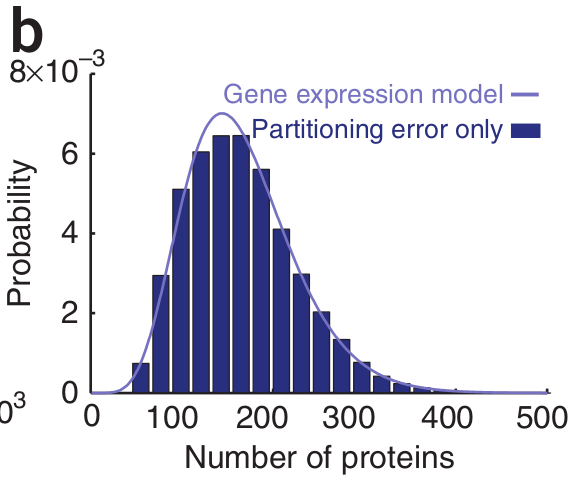
\includegraphics[width=0.5\textwidth]{fitting.png}\\
    \tiny \cite{huh11a}.
\end{figure}
\end{frame}

\iffalse
\begin{frame}
\frametitle{}
\begin{figure}[p]
    \centering
    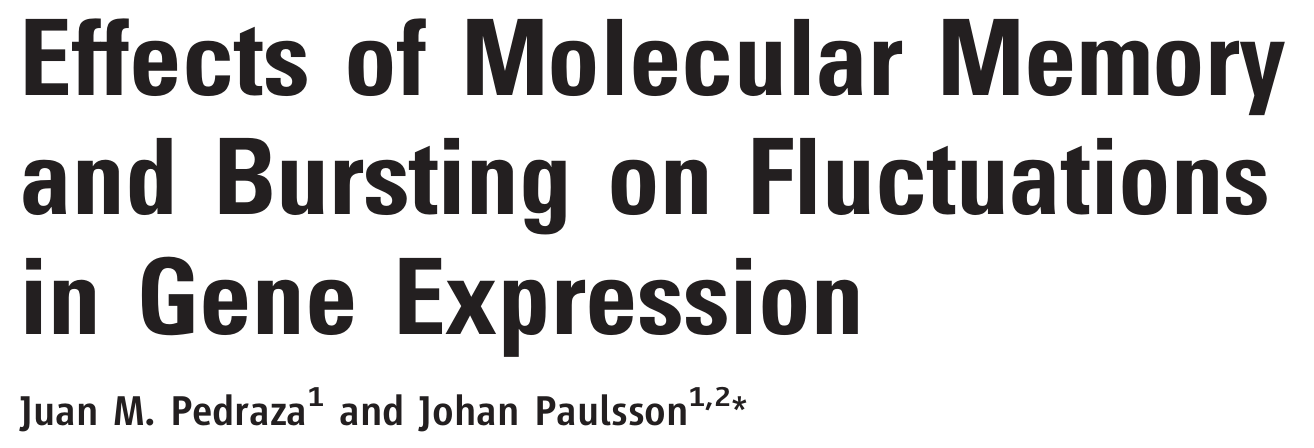
\includegraphics[width=0.5\textwidth]{pedraza08.png}\\
    \tiny \cite{pedraza08}.
\end{figure}

\begin{figure}[p]
    \centering
    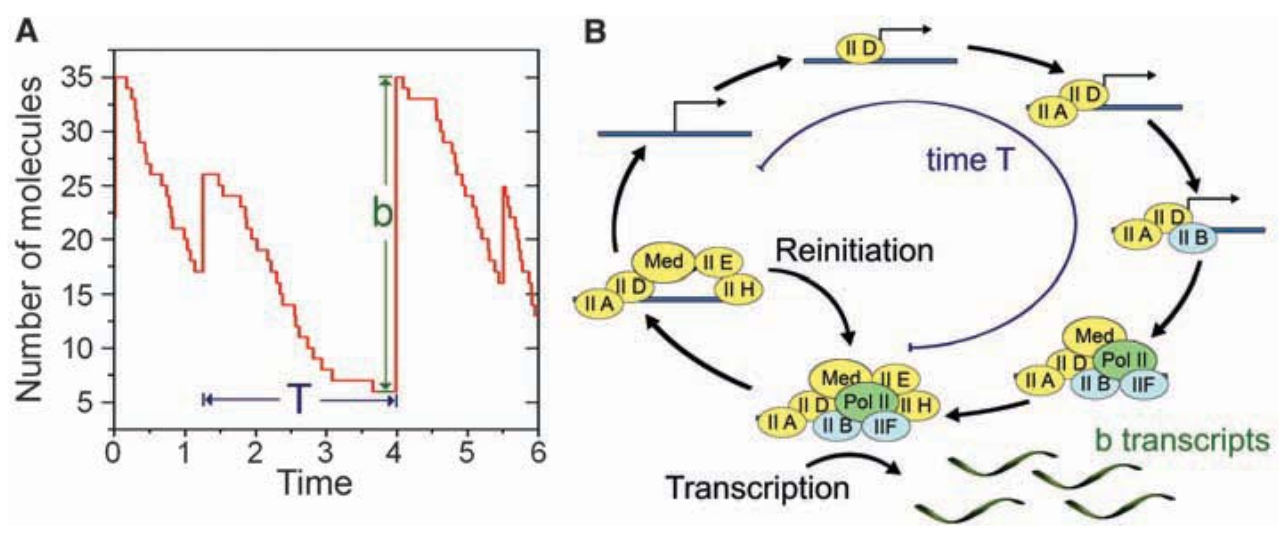
\includegraphics[width=0.6\textwidth]{bursting.png}\\
    \tiny \cite{pedraza08}.
\end{figure}
$$\frac{\sigma_p^2}{\langle p \rangle^2} = \frac{1}{\langle p \rangle} + \frac{1}{\langle r \rangle} \cdot \frac{\tau_r}{\tau_r + \tau_p} \cdot \frac{\langle b \rangle (\sigma_T^2/\langle T \rangle^2 + \sigma_b^2/\langle b \rangle^2) + 1}{2}$$
\end{frame}
\fi
\begin{frame}
\frametitle{Futuras investigaciones}
\begin{itemize}

\item Considerar las no-linealidades.
\item Considerar la din\'amica temporal del ruido.
\item Posibilidad de usar herramientas te\'oricas adicionales.

\end{itemize}
\end{frame}

\footnotesize{
\begin{frame}
\frametitle{Referencias}
\begin{thebibliography}{99}

\bibitem[Arkin et al., 1998]{arkin98} Arkin, A., Ross, J. \& McAdams H. H. (1998).
\newblock Stochastic Kinetic Analysis of Developmental Pathway Bifurcation in Phage $\lambda$-Infected Escherichia coli Cells.
\newblock \emph{Genetics} 149, 1633 -- 1648.

\bibitem[Cooper, 2000]{cooper00} Cooper, G. M. (2000).
\newblock The Cell, A Molecular Approach. 2nd Edition.
\newblock Sunderland (MA): Sinauer Associates.

\bibitem[Thattai \& van Oudenaarden, 2001]{thattai01} Thattai, M. \& van Oudenaarden, A. (2001).
\newblock Intrinsic noise in gene regulatory networks.
\newblock \emph{Proc. Natl. Acad. Sci. U.S.A.} 98(15), 8614 -- 8619.

\bibitem[Paulsson, 2004]{paulsson04} Paulsson, J. (2004)
\newblock Summing up the noise in gene networks.
\newblock \emph{Nature} 427, 415--418.

\bibitem[Kaern et al., 2005]{kaern05} Kaern, M., Elston, T. C., Blake, W. J. \& Collins, J. J. (2005).
\newblock Stochasticity in gene expression: from theories to phenothypes.
\newblock \emph{Nat. Rev. Genet.} 6(6), 451 -- 464.

\end{thebibliography}
\end{frame}

\begin{frame}
\frametitle{Referencias}
\begin{thebibliography}{99}

\bibitem[Pedraza \& van Oudenaarden, 2005]{pedraza05} Pedraza, J. M. \& van Oudenaarden, A. (2005).
\newblock Noise Propagation in Gene Networks.
\newblock \emph{Science} 307, 1965 -- 1969.

\bibitem[Paulsson, 2005]{paulsson05} Paulsson, J. (2005).
\newblock Models of stochastic gene expression.
\newblock \emph{Phys. Life Rev.} 2, 157--175.

\bibitem[Pedraza \& Paulsson, 2008]{pedraza08} Pedraza, J. M. \& Paulsson, J. (2008).
\newblock Effects of Molecular Memory and Bursting on Fluctuations in Gene Expression.
\newblock \emph{Science} 319, 339--343.

\bibitem[Huh \& Paulsson, 2011a]{huh11a} Huh, D. \& Paulsson, J. (2011).
\newblock Non-genetic heterogeneity from stochastic partitioning at cell division.
\newblock \emph{Nat. Genet.} 43, 95--100.

\bibitem[Huh \& Paulsson, 2011b]{huh11b} Huh, D. \& Paulsson, J. (2011).
\newblock Random partitioning of molecules at cell division.
\newblock \emph{Proc. Natl. Acad. Sci. U.S.A.} 108, 15004--15009.
\end{thebibliography}
\end{frame}
}
\end{document}
